\documentclass[10pt,twocolumn,twoside,final]{IEEEtran}

% cite package, to clean up citations in the main text. Do not remove.
\usepackage{cite}
\usepackage{lastpage,fancyhdr,graphicx}
\usepackage{amssymb,amsmath}
\usepackage{mathtools}

% Remove brackets from numbering in List of References
\makeatletter
\renewcommand{\@biblabel}[1]{\quad#1.}
\makeatother

% *** SUBFIGURE PACKAGES ***
\ifCLASSOPTIONcompsoc
  \usepackage[caption=false,font=footnotesize,labelfont=sf,textfont=sf]{subfig}
\else
  \usepackage[caption=false,font=footnotesize]{subfig}
\fi

\begin{document}

\title{Effective Dynamic Models of Metabolic Networks}


% author names and affiliations
% use a multiple column layout for up to three different
% affiliations
\author{\IEEEauthorblockN{Michael Vilkhovoy\IEEEauthorrefmark{1},
Mason Minot\IEEEauthorrefmark{2},
Jeffrey D. Varner\IEEEauthorrefmark{1}}\\
\IEEEauthorblockA{\IEEEauthorrefmark{1}School of Chemical Engineering, Purdue University, West Lafayette, IN 47907 USA}
\IEEEauthorblockA{\IEEEauthorrefmark{2}School of Chemical and Biomolecular Engineering, Cornell University, Ithaca, NY 14850 USA}
\thanks{Manuscript received December 1, 2012; revised September 17, 2014.
Corresponding author: J. Varner (email:jdvarner@purdue.edu).}}

\maketitle

\begin{abstract}
Mathematical models of biochemical networks are useful tools to understand and ultimately predict how cells utilize nutrients to produce valuable products.
Hybrid cybernetic models in combination with elementary modes (HCM EM) provides a route to model cellular metabolism.
However, this framework is limited to smaller networks due to the computational cost of calculating elementary modes and a high number of solutions for large networks.
In this study, we developed a hybrid cybernetic model in combination with flux balance analysis (HCM FBA) modes instead of elementary modes.
Flux balance analysis provides a sufficient number of modes (metabolic options) for the network to estimate experimental observations.
We show HCM FBA has comparable model performance to HCM EM for a hypothetical proof of concept metabolic network and for a reduced anaerobic \textit{E. coli} network.
HCM FBA was applied to a larger metabolic network where 29 FBA modes were computed, in contrast to over 66,000 elementary modes.  A sensitivity analysis was performed to reduce the number of FBA modes from 29 to 5. This reduction maintained a robust model performance to fit experimental observations.

\end{abstract}


\begin{IEEEkeywords}
Dynamic metabolic models, flux balance analysis, cybernetic models
\end{IEEEkeywords}

\section{Introduction}
Metabolic networks for simple organisms such as \textit{E. coli} contain thousands of reactions that are highly interconnected.
These organisms have the potential to be engineered to produce valuable products.
Mathematical models of biochemical networks are useful tools to understand and ultimately predict how cells utilize nutrients to produce valuable products.
Traditionally, Monod kinetics have been used as unstructured models to describe cell growth, substrate consumption, and product formation, but fail to account for intracellular metabolism\cite{shuler_book}.
Structured modeling approaches have made great progress to describe metabolic pathways including elementary mode analysis (EM)\cite{2006_vonKamp_Metatool}, metabolic flux analysis (MFA), flux balance analysis (FBA)\cite{2010_orth_NatBiotech}, dynamic FBA (DFBA) \cite{1994_varma_palsson_ApplEnvMicro,2002_Mahadevan_BiophysJ}, and hybrid cybernetic modeling (HCM) \cite{2008_kim_varner_ramkrishna_BiotechProg}.

Convex and constraints based analysis methods, such as EM, FBA and MFA,
describe intracellular metabolism using the stoichiometry of the biochemical networks and the pseudo-steady state assumption \cite{2010_orth_NatBiotech}.
EM analysis is a powerful tool to decompse a metabolic network into independent minimal pathways that are stoihiometrically and thermodynamically feasible.
However, elementary mode calculations are computational expensive and infeasible for genome scale networks\cite{2004_lee_varner_ko_ieee}.
FBA is frequently used to study genome-scale networks\cite{2010_orth_NatBiotech} and often results in good approximations for yields, however it fails to estimate intracellular metabolism due to its underdetermined solution space.
Compared with FBA, MFA has good estimations of intracellular metabolism, but is dependent on experimental data.
Just like FBA, HCM approaches cell metabolism as a resource allocation problem towards a specified objective. 
But HCM has multiple pathways to select from (elementary modes) and can use a combination of modes to direct its resources through the cell.
HCM has been shown to have comparable internal flux estimations to MFA and is able to estimate dynamic external fluxes with respect to experimental observations \cite{2008_kim_varner_ramkrishna_BiotechProg}.\
DFBA is able to account for dynamic external fluxes but fails to incorporate the regulatory processes involved with HCM without the use of boolean rules\cite{2001_covert_schilling_palsson}.
Despite the advantages of HCM, it is restricted to small networks due to the exponential increase of the number of elementary modes for large networks.
Recent work has been done to reduce the number of elementary modes by lumping modes into groups using complex weighting schemes and experimental data\cite{2010_song_ramkrishna}, however, HCM is still limited by EM decomposition.

In this study, we developed a hybrid cybernetic model in combination with flux balance analysis modes instead of elementary modes.
We show HCM FBA has comparable model performance to HCM EM for a hypothetical metabolic network and a reduced anaerobic \textit{E. coli} network.
HCM EM and HCM FBA were then applied to a large metabolic network. 
The number of elementary modes made it impractical to model with HCM EM, but HCM FBA was computationally feasible and performed well with respect to experimental observations.
Taken together, HCM FBA has comparable model performace to HCM EM and may be potentially applied to genome-scale networks which was a shortcoming of HCM EM.


\begin{figure}[!t]\centering
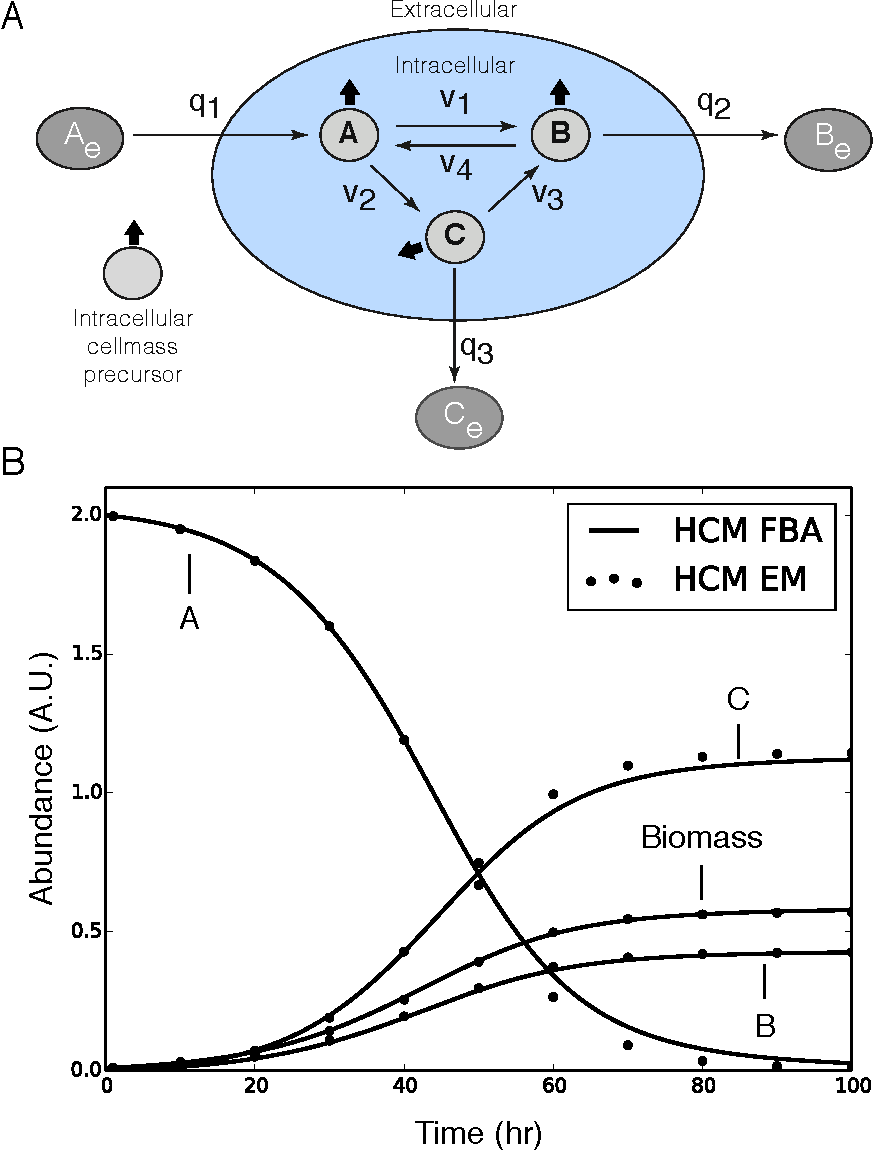
\includegraphics[width=0.40\textwidth]{./figs/Fig-1-GeneralModel-Results.pdf}
\caption{A: Proof of concept metabolic network with six metabolites and seven reactions.
Intracellular cellmass precursors $A,B$ and $C$ are balanced (no accumulation) while the extracellular metabolites ($A_{e},B_{e}$ and $C_{e}$) are not balanced (can accumulate). The blue-oval denotes the cell boundary, where $q_{j}$ denotes the jth flux across the boundaries ([mmol/gdw-hr]) and $v_{k}$ denotes the kth intracellular flux. B: Simulation of the extracellular metabolites using the FBA hybrid cybernetic approach (solid line) versus elementary modes (points) for the proof of concept metabolic network. FBA modes have comparable model performance compared to elementary modes.
}\label{fig:model-fitting}
\end{figure}

\section{Results}
The performance of HCM FBA was equivalent to HCM EM for a proof of concept metabolic network (Fig. \ref{fig:model-fitting}).
In the proof of concept metabolic network consisting of 6 metabolites and 7 reactions (Fig. \ref{fig:model-fitting}A), we calculated 6 elementary modes and 3 FBA modes.
Using the HCM EM modeling framework, concentration profiles were generated for the extracellular metabolites and artifical biomass (Fig. \ref {fig:model-fitting}B).
The kinetic parameters of HCM FBA were varied to fit the concentration profiles of the HCM EM model.
For this proof of concept model, HCM FBA was able to use fewer modes and kinetic parameters to mimic the simulation profiles of HCM EM.

The performance of HCM FBA was equivalent to HCM EM for a small model of anaerobic \textit{E. coli} metabolism (Fig. \ref{fig:ecoli}, left).
In the case, we demonstrated that HCM FBA has comparable model performance to a published HCM EM model \cite{2008_kim_varner_ramkrishna_BiotechProg}.
The metabolic network consisted of 12 reactions, where we calculated 9 elementary modes and 7 FBA modes.
The simulated HCM EM concentration profiles of biomass, substrate and fermentation products (Fig. \ref {fig:ecoli}A (dashed line)) were generated using the kinetic parameters and elementary modes reported\cite{2008_kim_varner_ramkrishna_BiotechProg}.
The kinetic parameters of HCM FBA were varied to fit the same experimental observations.
HCM FBA has 17 kinetic parameters while HCM EM has 21 kinetic parameters and both models resulted in similar fits to the experimental data (Fig. \ref {fig:ecoli}A).
HCM FBA had a slightly better fit on lactate than HCM EM.

\begin{figure}[!t]\centering
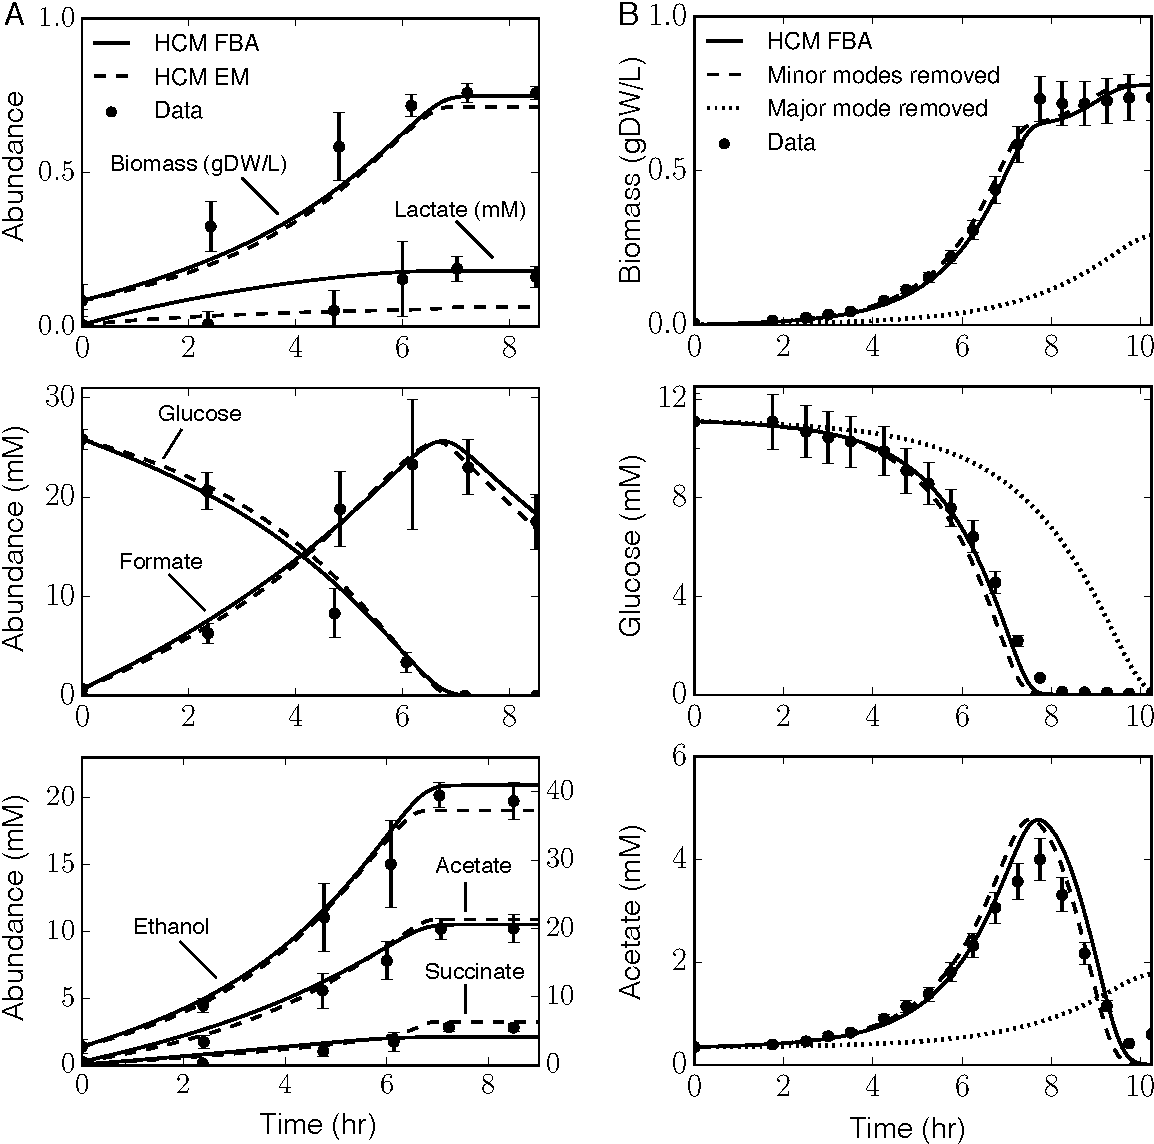
\includegraphics[width=0.48\textwidth]{./figs/Fig-2-Ecoli-SimulationResults.pdf}
\caption{A: Batch anaerobic \textit{E. coli} fermentation data versus simulation of the hybrid cybernetic model with FBA modes (solid line) and elementary modes (dashed line). (Experimental data from Kim et. al (2008)\cite{2008_kim_varner_ramkrishna_BiotechProg} with error bars representing 90\% confidence intervals.) B: Batch aerobic \textit{E. coli} fermentation data of glucose, acetate and cell density measurements versus simulation of the hybrid cybernetic model with FBA modes (solid line). Model performance is shown when minor modes (dashed) and a major mode (dotted) is removed from HCM FBA. (Experimental data from Varma \& Palsson (1994)\cite{1994_varma_palsson_ApplEnvMicro} with assumed 10\% error bars).}
\label{fig:ecoli}
\end{figure}

HCM FBA outperformed HCM EM for a large model of aerobic \textit{E. coli} metabolism (Fig. \ref{fig:ecoli}, right).
In the case, we demonstrated that HCM FBA is applicable for larger metabolic networks where elementary mode calculations increase exponentially.
A metabolic network\cite{2007_schuetz_etal_MolSysBio} of 98 reactions and 60 metabolites with the biomass reaction from Palsson's \textit{E. coli} core model\cite{2006_Palsson_model} was used.
We calculated over 66,000 elementary modes for this network and determined it was futile to model.
For the same network, we computed 29 FBA modes.
HCM FBA was simulated to fit cell density, glucose and acetate measurements for an aerobic \textit{E. coli} batch culture\cite{1994_varma_palsson_ApplEnvMicro} (Fig.\ref{fig:ecoli}B (solid line)).

Variance based sensitivity of aerobic \textit{E. coli} metabolism identified modes that were essential to biomass yield (Fig. \ref{fig:sensitivity}).
The analysis calculated the total order sensitivity indicies of all the kinetic parameters and enzyme initial conditions.
We used the sensitivity results as a simple systematic method to eliminate FBA modes to give the smallest number needed while maintaining good model performance.
Five FBA modes were determined to be significant by an arbitrary threshold of 0.00218.
The remaining 24 FBA modes were identified to be minor modes and insignificant.
The removal of the major mode, representing aerobic growth, (Fig, \ref{fig:ecoli}B (dotted line)) was detrimental to model performance, whereas the removal of the minor modes (dashed line) had little effect.

\begin{figure*}[!t]\centering
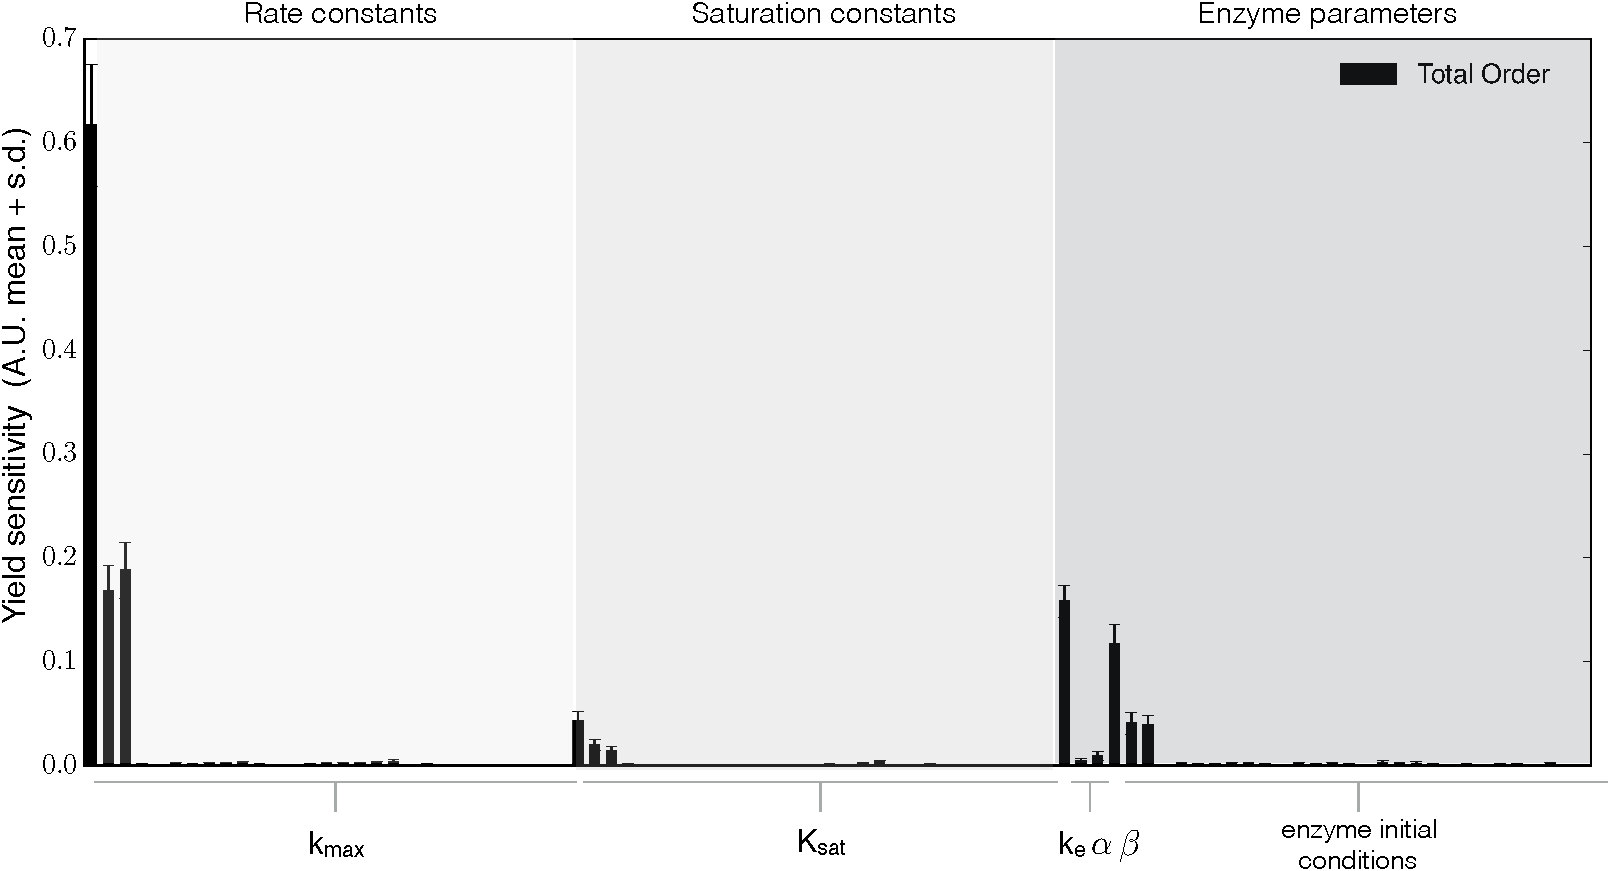
\includegraphics[width=0.85\textwidth]{./figs/Fig-3-Sensitivity-Results.pdf}
\caption{Total order variance based sensitivity analysis on biomass yield from glucose and acetate. Sensitivity indicies computed for rate constants, saturation constants and enzyme parameters. The most critical parameters are associated with mode 1 representing aerobic growth. (Error bars represent 95\% confidence intervals).
}
\label{fig:sensitivity}
\end{figure*}


\section{Discussion}
In this study, we developed a hybrid cybernetic model in combination with flux balance analysis modes instead of elementary modes.
First, we showed HCM FBA can have comparable model performance to HCM EM for a proof of concept metabolic network.
This judgement is based on the quality of fit of the model simulation to the observations.
Next, HCM FBA model performance was compared to an established HCM EM model\cite{2008_kim_varner_ramkrishna_BiotechProg} for an anaerobic culture of \textit{E. coli}.
HCM FBA had comparable fits to HCM EM on the fermentation data and a slightly better fit on lactate measurements.
Finally, HCM was applied to a larger metabolic network where 29 FBA modes were computed, in contrast to over 66,000 elementary modes.
HCM FBA was shown to have robust model performance only requiring 5 of the 29 FBA modes (selected by the sensitivity analysis) to fit experimental observations.

The hybrid cybernetic model is formulated to maximize substrate uptake based on cybernetic arguments.
Towards this objective, HCM uses a combination of modes to describe both the external and internal fluxes.
The internal fluxes still follow the pseudo steady state approximation applied in FBA, but HCM uses a combination of pathways.
HCM EM has been shown to have comparable internal flux estimates to MFA results\cite{2008_kim_varner_ramkrishna_BiotechProg}, this has not been shown for HCM FBA.
The HCM framework has been shown to predict dynamic external fluxes using both elementary and FBA modes.
While DFBA already has the capacity to estimate dynamic external fluxes, it requires \textit{a priori} knowledge and boolean rules to capture the diauxic phenomena \cite{1994_varma_palsson_ApplEnvMicro,2002_Mahadevan_BiophysJ,2001_covert_schilling_palsson}.
HCM overcomes this by incorparting the regulatory processes of substrate utilization based on its cybernetic arguments.
HCM EM has good model performance for reduced networks, but is impractical for larger networks.
HCM EM has been applied to a network with 67 reactions, requiring the elementary modes to be lumped into groups by complex weighting schemes and relying on experimental data\cite{2010_song_ramkrishna}.
A shortcoming of the HCM EM framework is that EM calculations are computationally expensive and the number of modes exponentially increases for larger networks \cite{2004_lee_varner_ko_ieee}.
In contrast, FBA does not have the computational burden associated with calculating elementary modes.
FBA is frequently used to study genome-scale networks\cite{2010_orth_NatBiotech} and can be used to generate modes for the HCM framework.
This opens up the possibility of genome scale cybernetic models.

HCM FBA provides a practical and feasible approach to model large networks where elementary modes fail.
The disadvantage of HCM FBA is it requires \textit{a priori} knowledge of the inputs into the metabolic network.
FBA modes do not have the thorough information as elementary modes, but provide sufficient pathways to model experimental observations.
%HCM FBA may also be applied to mammalian networks, as long as FBA accounts for compartmentalization within mammalian systems.

\section{Materials and Methods}

\noindent\subsubsection*{HCM FBA method.}
The model was constructed using the hybrid cybernetic approach of Kim et al.\cite{2008_kim_varner_ramkrishna_BiotechProg}.
The abundance of extracellular species $i$ ($x_{i}$) is governed by:
\begin{equation}
	\frac{dx_{i}}{dt}  =  \sum_{j = 1}^{\mathcal{R}}\sum_{l = 1}^{\mathcal{L}}\sigma_{ij}z_{jl}r_{l}\left(\mathbf{e},\mathbf{k},\mathbf{s}\right)c \qquad{i=1,\hdots,\mathcal{M}}
\end{equation}
where $\mathcal{R}$ and $\mathcal{M}$ denotes the number of reactions and extracellular species in the model, and $\mathcal{L}$ denotes the number of modes.
The quantity $\sigma_{ij}$ denotes the stoichiometric coefficient for species $i$ in reaction $j$ and
$z_{jl}$ denotes the normalized flux for reaction $j$ in mode $l$.
If $\sigma_{ij}>0$, species $i$ is produced by reaction $j$, if $\sigma_{ij}<0$, species $i$ is consumed by reaction $j$, while $\sigma_{ij} = 0$ indicates species $i$ is not connected with reaction $j$.
Extracellular species balances were subject to the initial conditions $\mathbf{x}\left(t_{o}\right) = \mathbf{x}_{o}$ determined from experimental data.
The $r_{l}\left(\mathbf{e},\mathbf{k},\mathbf{s}\right)$ term denotes the regulated uptake rate of mode $k$, and was written as the product of a kinetic term ($\bar{r}_{l}$) and a cybernetic control variable for enzyme activity ($v_{l}$), $r_{l}\left(\mathbf{e},\mathbf{k},\mathbf{s}\right) = \bar{r}_{l}v_{l}$, where $\mathbf{e}$ denotes the enzyme level for each mode which become additional state variables, $\mathbf{k}$ ($\mathcal{K}\times{1}$) denotes the unknown kinetic parameter vector, and $\mathbf{s}$ denotes the substrate utilized. The reaction rate followed Michaelis-Menten kinetics. The abundance of the enzyme species is governed by:

\begin{equation}
	\frac{de_{l}}{dt}  = \alpha_{l} + r_{E,l}\left(\mathbf{k},\mathbf{s}\right)u_{l} - \left(\beta_{l}+r_{G}\right)e_{l}
\end{equation}
where $\alpha_{l}$ denotes the specific rate of constitutive enzyme synthesis for enzyme l, $r_{E,l}\left(\mathbf{k},\mathbf{s}\right)$ denotes the specific rate enzyme synthesis for enzyme l, and $u_{l}$ denotes the cybernetic variable controlling the synthesis of enzyme l.
The term $\beta_{l}$ denotes the rate constant governing enzyme degradation, and $r_{G}$ denotes the growth rate through all modes.
The specific rate of enzyme synthesis was modeled using saturation kinetics.
All enzyme initial conditions were set to 0.9 for the anaerobic case, and 0.8 for the aerobic case.

\begin{equation}
	r_{G}  = \sum_{l = 1}^{\mathcal{L}}z_{\mu l}r_{l}\left(\mathbf{e},\mathbf{k},\mathbf{s}\right)
\end{equation}
where $z_{\mu l}$ denotes the growth flux $\mu$ through mode $l$.
The cybernetic control variables, $u_{l}$ and $v_{l}$, control the synthesis and activity of each enzyme for each mode using the matching and proportional laws\cite{2007_young_ramkrishna_BiotechProg}.
They are formulated to maximize the overall substrate uptake rate through each mode.

\begin{equation}
	u_{l}  = \frac{z_{s,l}\bar{r}_{l}}{\sum_{l = 1}^{\mathcal{L}}z_{sl}\bar{r}_{l}}
\end{equation}
\begin{equation}
	v_{l} = \frac{z_{s,l}\bar{r}_{l}}{\max_{l=1} z_{sl}\bar{r}_{l}}
\end{equation}
where $z_{sl}$ denotes the uptake flux of substrate $s$ through mode $l$.
In the anaerobic case we followed the assumption of Young's thesis\cite{2005_Young} and Kim et al.\cite{2008_kim_varner_ramkrishna_BiotechProg} that formate decomposition occurs only outside the network (applicable for strain GJT001).
Therefore its enzyme activity was assumed to be at its maximum level of unity.
The reaction rate for formate was also modified following Kim et al.\cite{2008_kim_varner_ramkrishna_BiotechProg}

\subsubsection*{Elementary Flux Mode Analysis}
The elementary flux modes were calculated using METATOOL 5.1\cite{2006_vonKamp_Metatool} for all networks.
The input file requires the conditions for reversibility/irreversibility reactions and intracellular/extracellular metabolites to be specified.

\subsubsection*{Flux Balance Analysis}
Flux balance analysis determines an optimal flux vector $\mathbf{w}$ subject to the stoichiometric matrix and flux constraints that maximizes/minimize a specified objective.
FBA modes were defined as the solution flux vector through the network.
FBA is formulated by the follwoing:

\begin{equation}
 \begin{multlined}
	\qquad \qquad \qquad \max_{\boldsymbol{w}}{} \! \left( w_{obj} = \boldsymbol{c}^T \boldsymbol{w} \right) \\
	\mathrm{Subject \; to:}
	 \; \; \mathbf{S}\mathbf{w}=0 \mathrm{\; and \;} \mathbf{S_{x}}\mathbf{w} = \mathbf{b} \\
\alpha_i \leq w_i \leq \beta_i  \qquad
 \end{multlined}
\end{equation}
where $\boldsymbol{c}$ is a vector of weights indicating how each flux contributes to the objective; $\alpha_i$ and $\beta_i$ are the lower and upper limits for the individual flux values, respectively.
The stoichoimetric matrix $\mathbf{S}$ denotes the intracellular network where intracellular metabolism has a psuedo steady state approximation.
$\mathbf{S_{x}}$ denotes the extracellular metabolic network and $\mathbf{b}$ denotes the exchange flux across the cell membrane.
FBA was solved using linear programming by a GNU Linear Programming Kit, GLPK version 4.52.
For each mode, the objective was set to maximize either the growth flux or each fermentation byproduct flux from a specified substrate.
Multiple modes were calculated for each objective flux by allowing the oxygen and nitrate uptake rates to be either nonexistent or its maximum.
In the aerobic case, oxygen and nitrate uptake rates were constrained to allow a maximum flux of 10 mM/gDW$\cdot$hr and 0.05 mM/gDW$\cdot$hr, respectively.
Each flux vector was normalized by the growth flux, or by the specified objective flux.

\subsubsection*{Sensitivity Analysis}
The variance based sensitivity analysis\cite{2010_saltelli} was done using SALib, an open source Python library. The sensitivity analysis identified key parameters that were influential on our specified model output of biomass yield. All model parameters used in the Sobol sensitivity analysis varied between 50\% lower and higher than the optimal values obtained from parameter identification, except enzyme initital conditions which varied between 0 and 1. The sample space was set to 1000 and 182,000 parameter sets were generated from the pseudo-random Sobol sequence.

\subsubsection*{Estimation of model parameters}
Model parameters were estimated by minimizing the difference between simulations and experimental measurements (squared residual):

\begin{equation}\label{eqn:objective-function}
	\min_{\mathbf{k}} \sum_{\tau=1}^{\mathcal{T}}\sum_{j=1}^{\mathcal{S}}\left(\frac{\hat{x}_{j}\left(\tau\right) - x_{j}\left(\tau,\mathbf{k}\right)}{\omega_{j}\left(\tau\right)}\right)^{2}
\end{equation}

where $\hat{x}_{j}\left(\tau\right)$ denotes the measured value of species $j$ at time $\tau$, $x_{j}\left(\tau,\mathbf{k}\right)$ denotes the simulated
value for species $j$ at time $\tau$, and $\omega_{j}\left(\tau\right)$ denotes the experimental measurement variance for species $j$ at time $\tau$.
The outer summation is with respect to time, while the inner summation is with respect to state. We minimized the model residual using simulated annealing.

% References -
\bibliographystyle{naturemag_noURL}
\bibliography{Paper_v1}

\end{document}
\grid
